\documentclass[22pt]{beamer}

\usepackage{templates/beamerthemekit}
\usepackage{graphicx}
\usepackage[utf8]{inputenc}
\usepackage[ngerman]{babel}

\usepackage{tikz}

\title[OSIP]{OPC UA Simulator for Industrial Plants}
\subtitle{PSE Projekt}
\author{M. Armbruster, D. Kahles, H. Lehmann, M. Schwarzmann, N. Wilhelm}

\titlelogo{icon}

\begin{document}

\selectlanguage{ngerman}

%title page
\begin{frame}
\titlepage
\end{frame}

\begin{frame}{Wofür benötigt man OSIP?}
\begin{figure}[ht!]
\centering
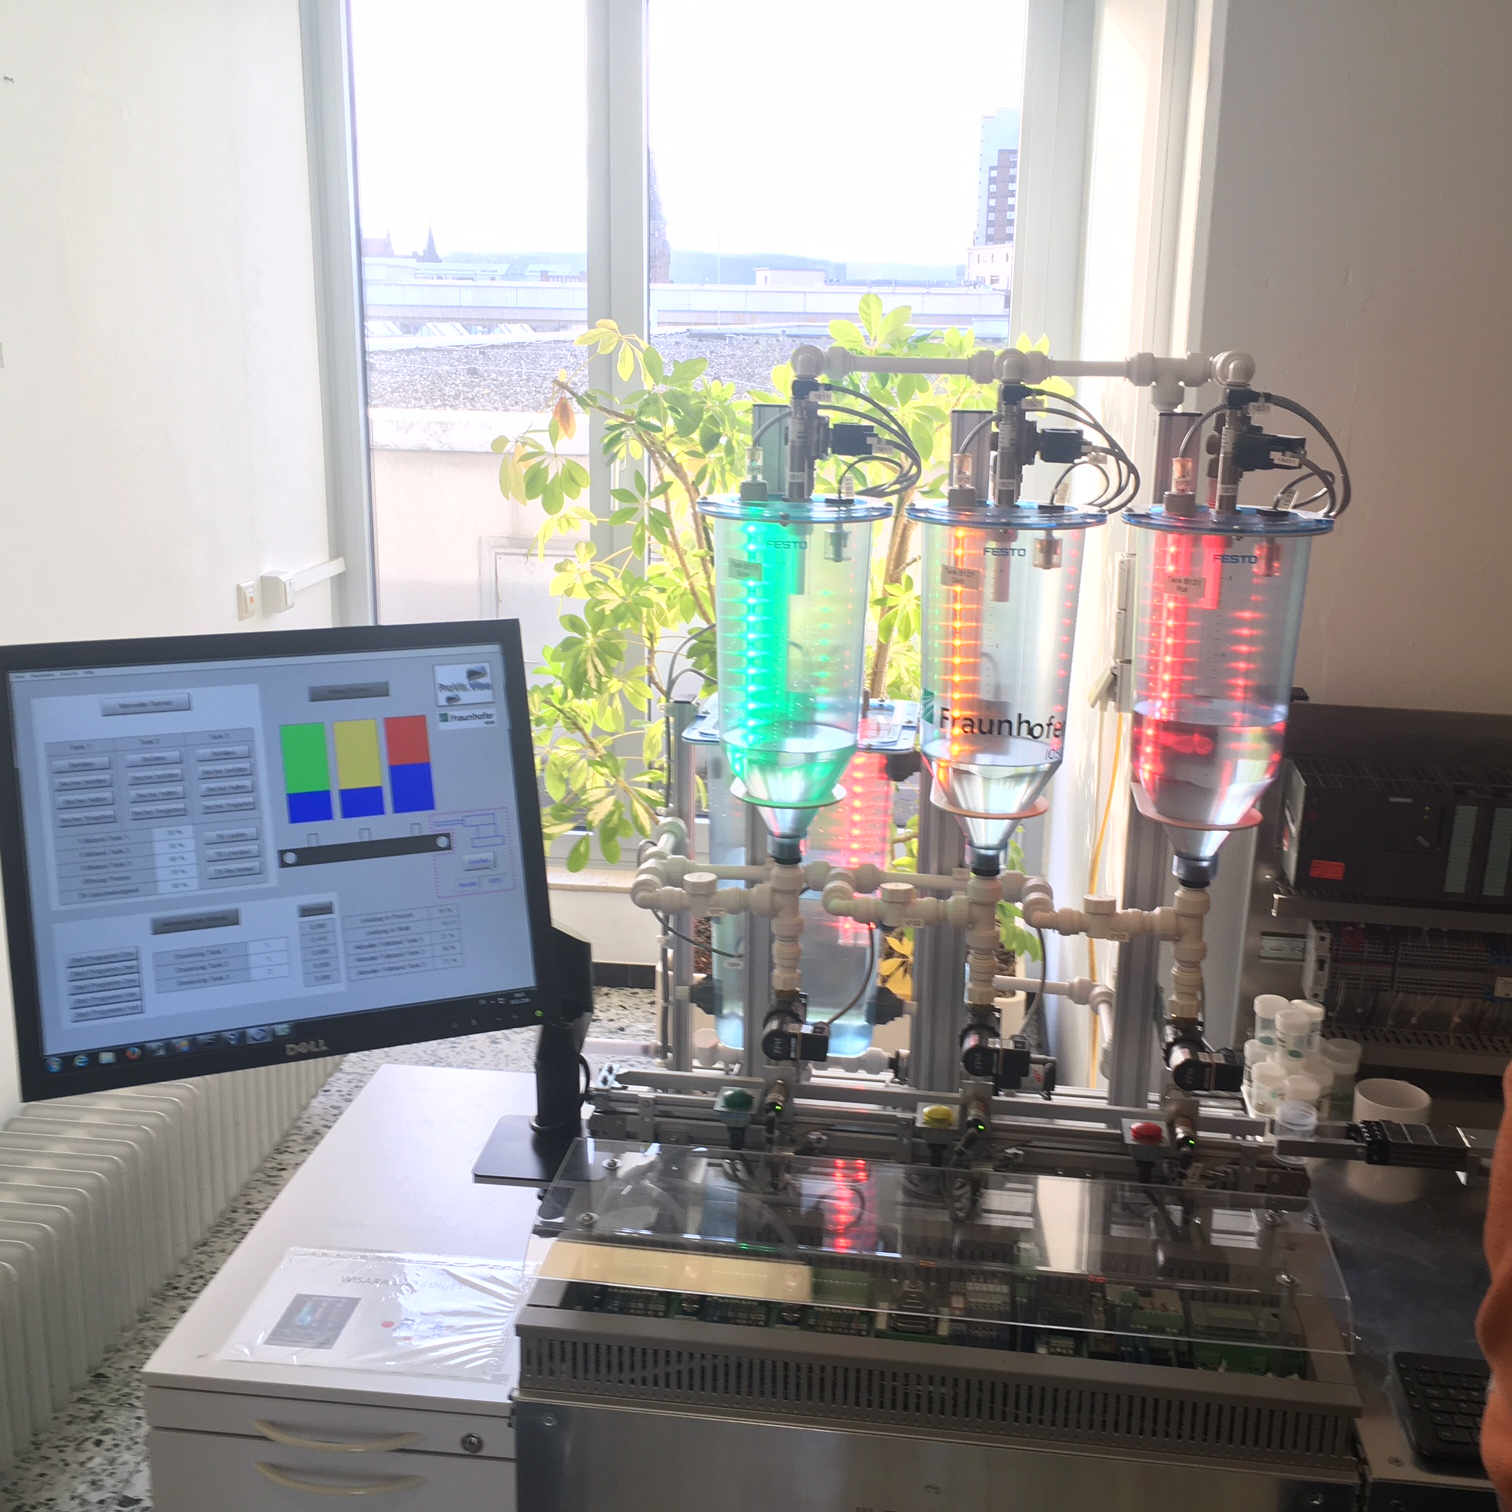
\includegraphics[height=\textheight,width=\textwidth,keepaspectratio=true]{Demoanlage_IOSB.jpg}
\end{figure}
\end{frame}

\begin{frame}{Was ist OSIP?}
\begin{itemize}[<+->]
 \item zwei Anwendungen: \emph{Simulation} eines chemischen Produktionsprozesses mit vier Tanks und \emph{Überwachungskonsole}
 \item Kommunikation ausschließlich über OPC UA Protokoll
 \item Anwendungen per Netzwerk auf getrennten Computern lauffähig
\end{itemize}
\end{frame}

{ % all template changes are local to this group.
    \setbeamertemplate{navigation symbols}{}
    \begin{frame}[plain]
        \begin{tikzpicture}[remember picture,overlay]
            \node[at=(current page.center)] {
                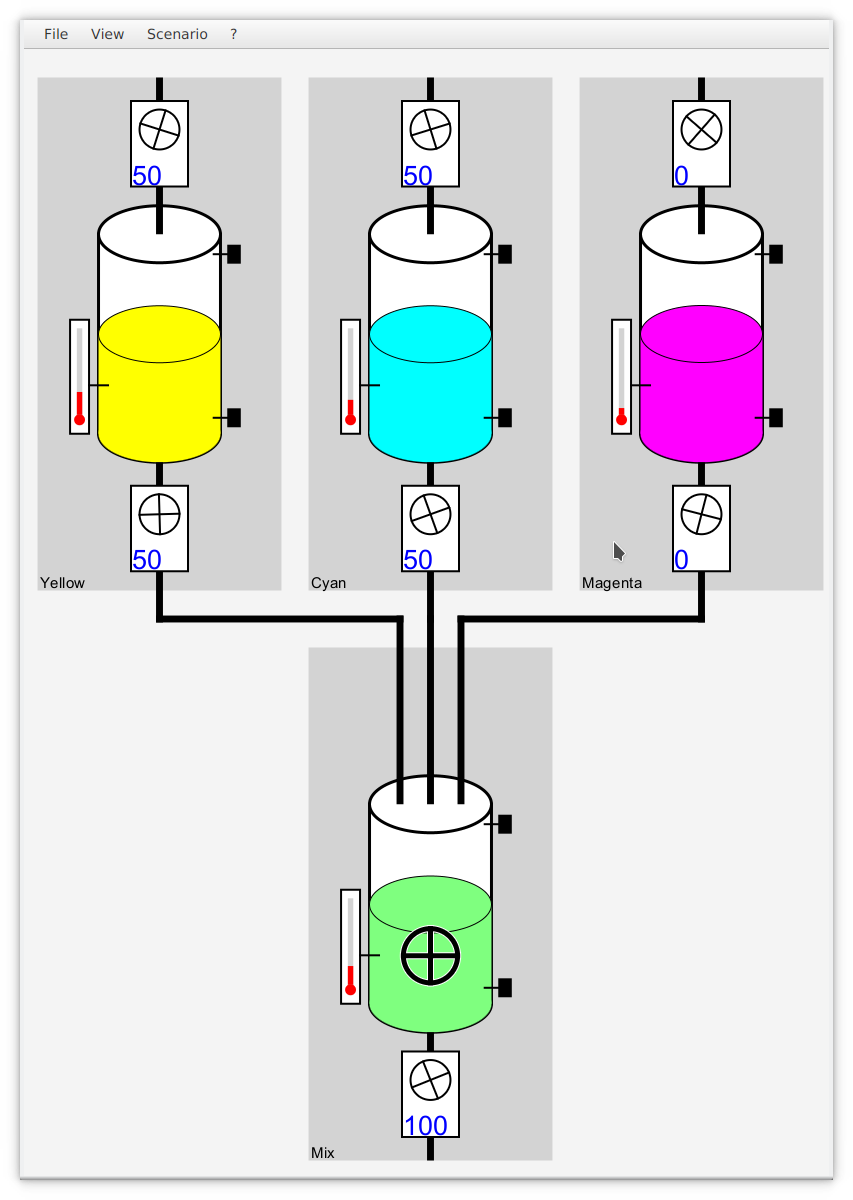
\includegraphics[height=\paperheight,width=\paperwidth,keepaspectratio=true]{ScreenshotSimulation.png}
            };
        \end{tikzpicture}
     \end{frame}
     
    \begin{frame}[plain]
        \begin{tikzpicture}[remember picture,overlay]
            \node[at=(current page.center)] {
                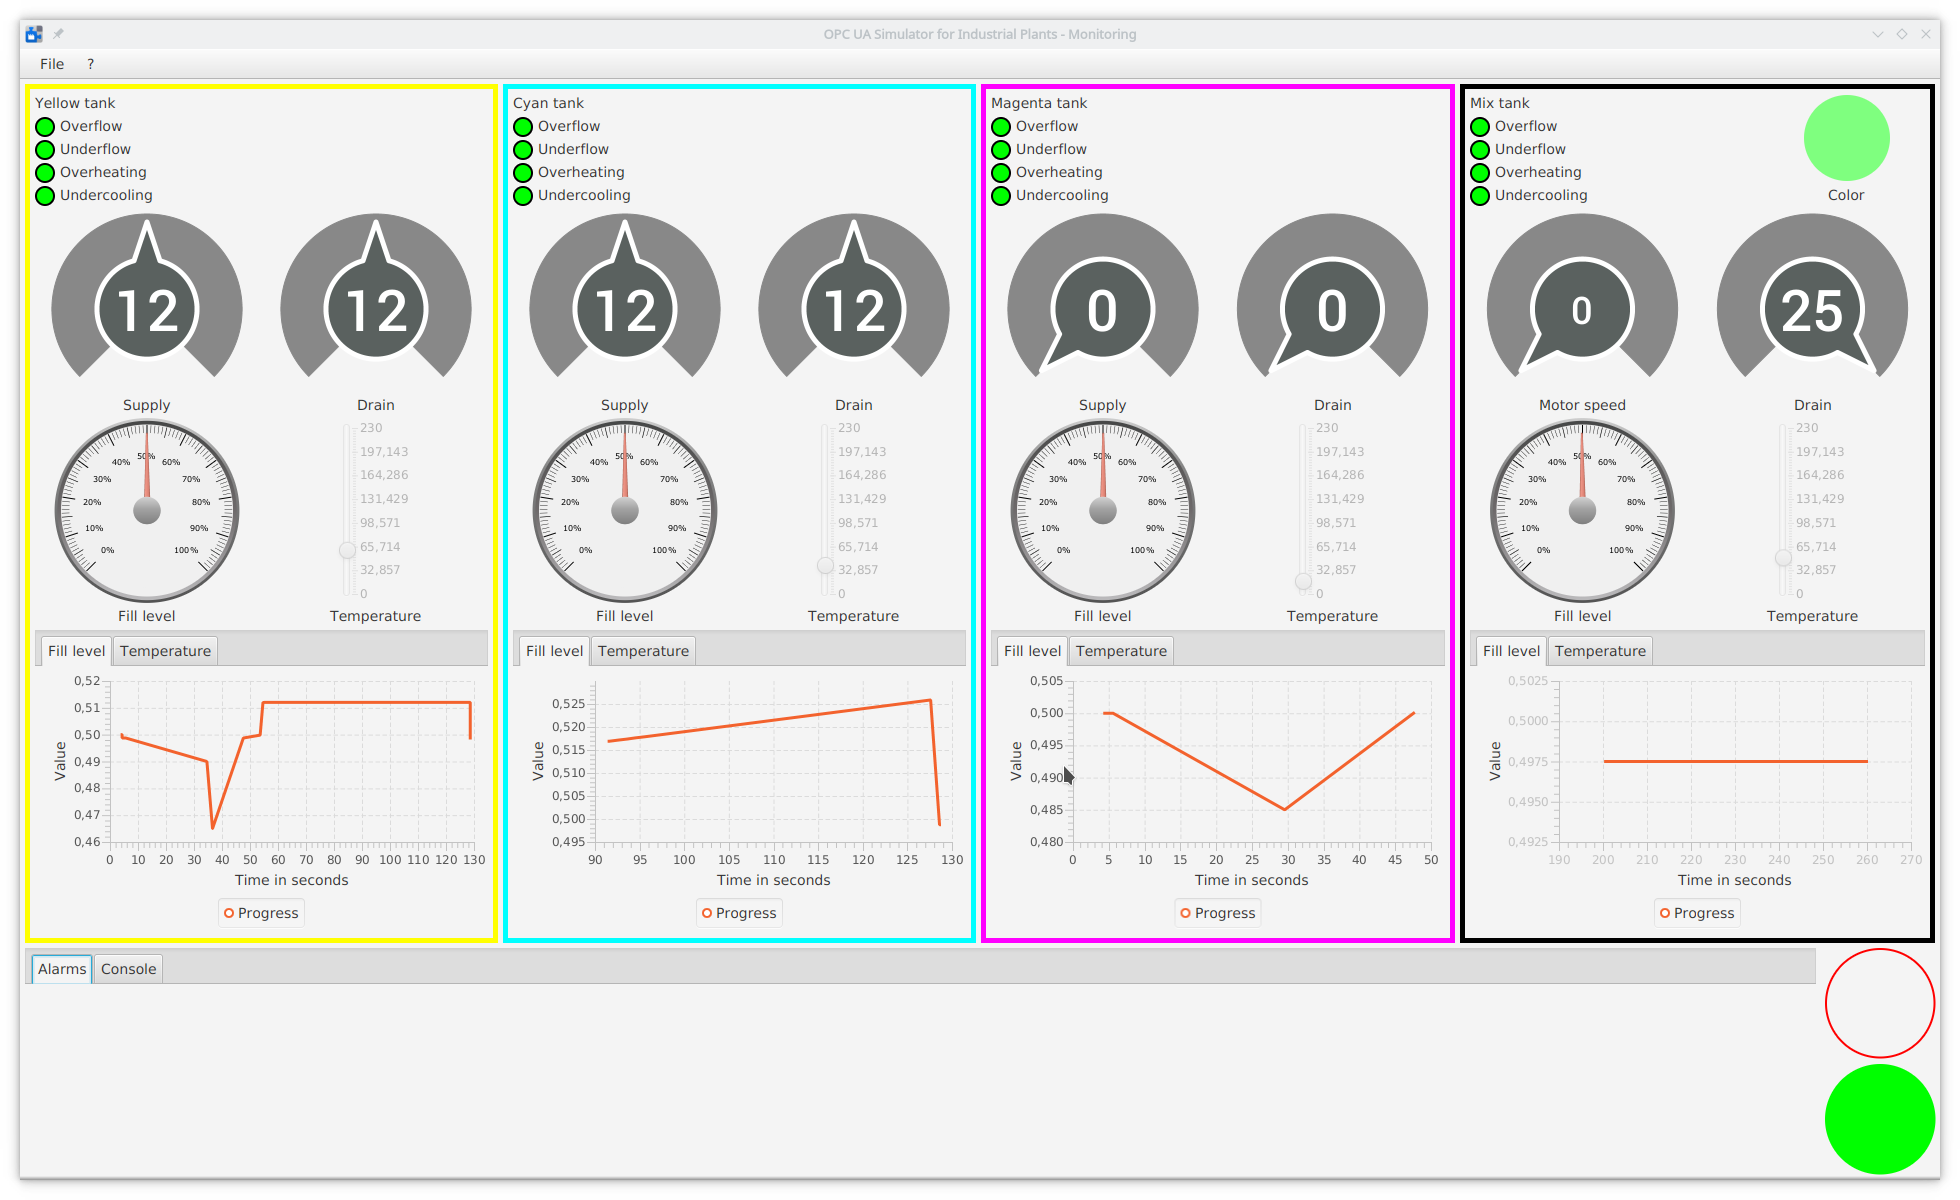
\includegraphics[height=\paperheight,width=\paperwidth,keepaspectratio=true]{ScreenshotMonitor.png}
            };
        \end{tikzpicture}
     \end{frame}
}

\begin{frame}{Verwendete Technologien}
\begin{itemize}[<+->]
 \item OPC UA Protokoll nicht selbst implementieren $\rightarrow$ Open Source Implementierung \emph{Milo}
 \item Programmiersprache: \emph{Java}
 \item Bauen des Projekts: \emph{Maven}
 \item Entwicklung der GUI: \emph{JavaFX}
 \item \emph{Git} mit Codereview und CI auf \emph{GitHub.com}
 \item Plattformen: Ubuntu 16.04 und Windows 10
 \item Unter Ubuntu: einfaches starten in Docker Containern
\end{itemize}
\end{frame}

\begin{frame}{Was haben wir bis jetzt?}
\begin{itemize}[<+->]
 \item circa 800 Commits
 \item Verschiedene Entwurfsmuster
 \begin{itemize}
  \item Model-View-Controller
  \item Fassade
  \item Strategie
  \item ...
 \end{itemize}
 \item Circa 15.000 LOC, davon 7500 SLOC
 \item Fast alle geplanten Features umgesetzt
\end{itemize}
\end{frame}

\begin{frame}{It's Showtime}
\centering
\huge
\textbf{Demo}
\end{frame}

\begin{frame}{Resümee}
\begin{itemize}[<+->]
 \item Code Review und CI vermeiden viele Probleme
 \item Controller (und generell Implementierungsphase) aufwändiger als gedacht
 \item Entwurf bei den Schnittstellen zwischen Controller und View unvollständig
 \item Unittesten der Nicht-GUI Komponenten nützlich
 \item Zeitplan bei der Implementierung nicht ganz eingehalten
\end{itemize}
\end{frame}

\end{document}
